\section{CONTACT CONFIGURATION}
\normalsize{The \acrshort{ECRH} \acrshort{TZM} reflector tile is an assembly composed of different parts held together using a specific bolting system. It is crucial to correctly set the contacts of the parts to accurately model the real life phenomena. Contacts are a quite complex concept and introduce lots of different problematics when modelling them. They can have all sorts of properties such as the number of degrees of freedom and possible movement or a specific heat transfer coefficient. In the case of the reflector tile assembly, the contact are of different types, mainly unidirectional and bonded.}
\\
\break
\normalsize{\indent Mathematically, contacts such as unidirectional contacts introduce discontinuities and nonlinearities that can influence convergence of the calculations. The methods chosen for the contacts will impact the speed and stability of the calculations, this is why the settings of the contacts were chosen with great care to avoid faulty calculations and improbable results.}
\\
\break
\normalsize{\indent In real life, the \acrshort{TZM} tile is placed on top of the \acrshort{Sigraflex} thermal gasket. The \acrshort{CuCrZr} heat sink is placed in the other side of the \acrshort{Sigraflex} thermal gasket. Those two contacts (tile/thermal gasket and thermal gasket/heat sink) are all unidirectional and frictional. The \acrshort{SS} cooling pipe is brazed onto the \acrshort{CuCrZr} heat sink. This bonds the heat sink and the cooling pipe together. For this contact, it is assumed that both are thermally perfectly bonded, meaning that the temperature on one part at the boundary is the same as the temperature on the contact boundary of the other part. In some cases, this brazed contact will have a reduced contact area to simulate a "bad" brazing and assess the impact of a worsen thermal contact.}
\\
\break
\normalsize{\indent The bolting system is a complex assembly and interacting parts composed of the \acrshort{TZM} bolts, the \acrshort{TZM} holding pins, the \acrshort{SS} nut, the INCONEL Belleville washers. The reflector tile has a closed plasma-facing surface. The bolts thus need to the held in the tile, and because it is not possible to directly use the reflector tile to fix the bolt. It was decided to design \acrshort{TZM} holding pins screwed on the side of the reflector tile. Those holding/retaining pins are designed to retain the head of the bolt using fingers. In total, 8 of such pins are assembled in the reflector tile. The holding pin/reflector tile connection is threaded but it was deemed acceptable to consider it bonded. The contact between the holding pins and the bolts are, however, unidirectional and frictional. The contact nut to bolt is also threaded but is considered bonded in the model. To accomodate for possible thermal expansion and deformation of the parts while still assuring thermal contact between the \acrshort{TZM} reflector tile and the \acrshort{CuCrZr} heat sink, as stack composed of three INCONEL Belleville washers acting as a spring, putting pressure on the reflector tile and maintaining thermal contact. The washers push on the \acrshort{CuCrZr} heat sink. All those contacts (nut/washer, and washer/heat sink) are considered to be unidirectional and frictional. The contact washer to washer is technically frictional but for modelling and solving reasons, they will be bonded at the outer perimeter, they still can rotate but not move.}

\subsection{Initial contact setup}
\normalsize{Initially, the early calculations only included (all contacts bonded):
\begin{itemize}
    \item The \acrshort{TZM} tile
    \item The \acrshort{Sigraflex} thermal gasket.
    \item The \acrshort{CuCrZr} heat sink.
    \item The \acrshort{SS} cooling pipe.
  \end{itemize}
This was done to test the modelling of the tile assembly and the bonding of the parts together. While this wasn't the most accurate model, the thermal claculations didn't need and more complex setup, and for the initial calculations, heat transfer was assumed to be perfect. The idea was then to add the bolting system. This means that the complex mechanical interaction between the boltins parts, especially the stack of Belleville washers needed to be modelled. A global assembly model was thus developed to implement the bolting system on the nature of the contacts and the modelling choices stated earlier.}
\\
\break
\normalsize{\indent It is now possible to establish a contact model for the whole assembly:}
\\
\break
\begin{figure}[h!]
  \label{fig_4_1_0} 
  \centering
  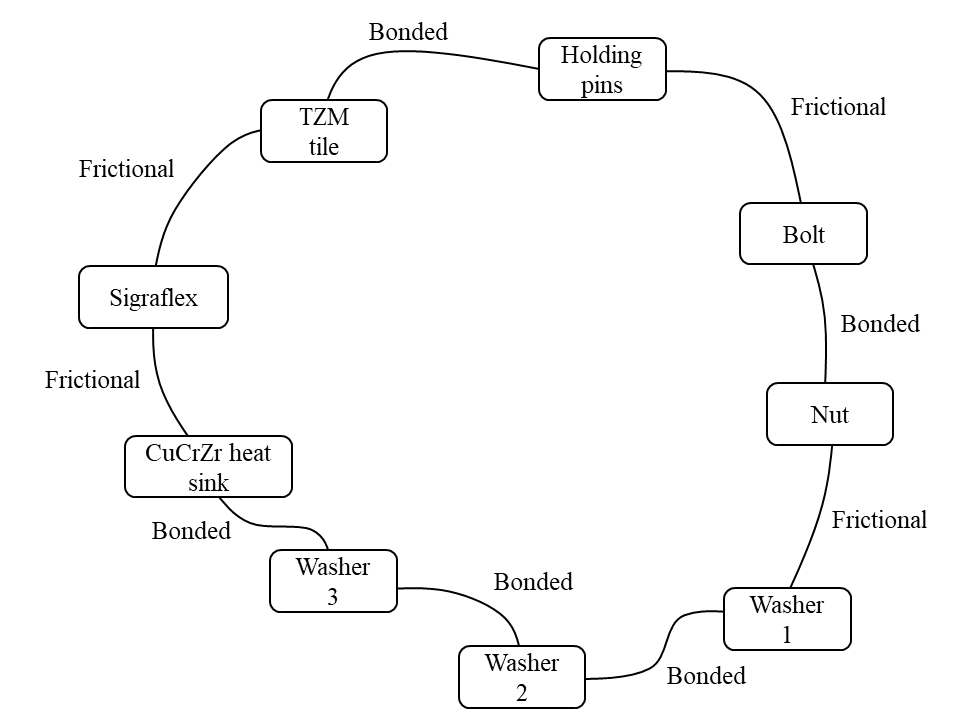
\includegraphics[width=.9\textwidth]{figures/contacts.png}
  \caption{\it Contact configuration for thermal and structural analysis}
\end{figure}
\\
\break
\normalsize{This model is acceptable but will be sometimes modified to assess the impact of the contact modelling.}
\\
\break
\normalsize{\indent When setting up the contacts in ANSYS\textsuperscript{\textregistered}, it is important to check for gaps of penertrations to avoid clipping issues. The status of the contact on a flat surface to surface contact should be consistent to avoid solving issues.}
\begin{figure}[h!]
  \label{fig_4_1_0} 
  \centering
  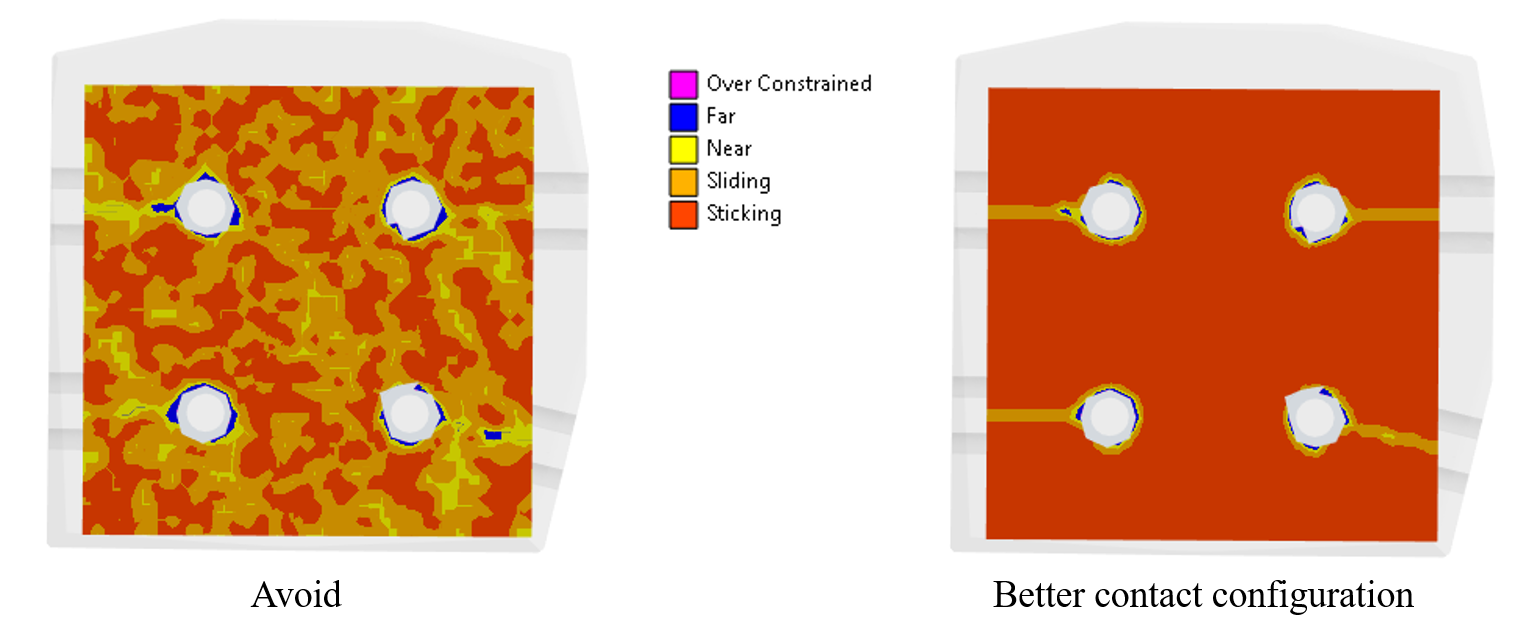
\includegraphics[width=0.8\textwidth]{figures/wonrgvsrightcs.png}
  \caption{\it Contact status comparison}
\end{figure}
\\
\break
\normalsize{\indent Such inconsistent contacts can make the calculation unstable and potentially prevent good results. Contact offset can be used to {\it"close"} the gap of the contacts allowing a better contact onfiguration. Contact methods can also be modified to other formulations all having their own use cases. For bonded contact and frictional contact, programmed controlled is most used. MPC can also be used for bonded contact, it usually blocks all degrees of freedom using constrain equations. Thermal contact is considered perfect because of the brazing. It is assumed that the heat conduction is really high and the modelling is not possible without data.}
\subsection{Field coupling and contact configuration}
\normalsize{Contact are complex phenomena that can be dependant on multiples fields. In the case of thermal-structural analysis, temperature and displacement fields can have an influence on the contact status of a given contact (ie. the break of contact preventing heat conduction). In chapter \ref{ch_5.4}, field coupling is used to model the loss of contact between the heat sink and the Sigraflex. It is discussed how manual update of the contact configuration can be of use to assess the need for full field coupling. In the case of too complex }
\\
\break
\normalsize{\indent For coupled field calculations (ie. thermal-structural), the elements used have more degrees of freedom (in this case these are displacement and temperature). The problem becomes large and convergence issues arise. It was decided to remove the bolting system as a first approach. The bonding of the \acrshort{Sigraflex} thermal gasket and the \acrshort{CuCrZr} heat sink was done in order to simplify the model and allow better if not convergence at all.}
\newpage